\documentclass{beamer}
\usepackage[utf8]{inputenc}
\usepackage[T1]{fontenc}
\usepackage[english]{babel}
\usepackage[babel=true]{csquotes}
\usepackage{graphicx}
\usepackage[export]{adjustbox}
\usepackage{amsmath}
\usepackage{algorithm2e}
\usepackage{hyperref}
\usepackage{listings}
\usepackage[toc,page]{appendix}
\usepackage[backend=biber,style=alphabetic]{biblatex}


\graphicspath{ {../images/} }
\usetheme{Copenhagen}
\setbeamertemplate{page number in head/foot}[totalframenumber]
\lstset{
    basicstyle=\ttfamily,
    breaklines=true,
    showstringspaces=false,
    keywordstyle=\color{blue},
}


\title{Numerical stability and fast-math}
\subtitle{Speeding up LHCb software through compilation optimization}
\author{Oscar Buon}


\begin{document}

\begin{frame}
    \centering
    \begin{minipage}{0.2\textwidth}
        
\includegraphics[width=\textwidth]{logo_ISIMA_INP.png}
    \end{minipage}\hfill
    \begin{minipage}{0.2\textwidth}
        
\includegraphics[width=\textwidth]{logo_CERN.png}
    \end{minipage}\hfill
    \begin{minipage}{0.2\textwidth}
        
\includegraphics[width=\textwidth]{logo_LHCb.png}
    \end{minipage}

    \maketitle

    Supervisor: Sebastien Ponce
\end{frame}

\part{Body}

\begin{frame}
    \frametitle{Table of contents}
    \tableofcontents
\end{frame}

\section{Introduction}

\begin{frame}
    \tableofcontents[currentsection]
\end{frame}

\subsection{Floating-point arithmetic}

\begin{frame}
    \frametitle{Floating-point arithmetic}

    \begin{displaymath}
        \begin{split}
            (0.75)_{10} & = (+ 7.5 \times 10^{-1})_{10} \\
            & = (+11 \times 2^{-2})_{2} \\
            & = (\underbrace{+}_{sign} \underbrace{1.1}_{mantissa} \times 2^{\overbrace{-1}^{exponent}})_{2} = (0.11)_{2}
        \end{split}
    \end{displaymath}
\end{frame}

\begin{frame}
    \frametitle{Non-nominal case}

    \begin{displaymath}
        \begin{split}
            (0.8)_{10} & \approx (1.1001100110011001101 \times 2^{-1})_{2} \\
            & \approx (0.80000019073486328125)_{10}
        \end{split}
    \end{displaymath}

    The representation is an approximation, because the number of bits is limited.
\end{frame}

\subsection{IEEE 754}

\begin{frame}
    \frametitle{IEEE 754}

    \begin{itemize}
        \item 32 bits ($\sim 7.2$ digits) and 64 bits ($\sim 15.9$ digits) formats ;
        \item Special rules:
              \begin{itemize}
                  \item Subnormal numbers (numbers very close to $0$) ;
                  \item Special values: -Inf, +Inf, NaN ;
                  \item Rounding rules ;
                  \item Exception handling ;
              \end{itemize}
        \item We should always consider floats as approximations !
    \end{itemize}
\end{frame}

\section{Correctness of some computations}

\begin{frame}
    \tableofcontents[currentsection]
\end{frame}

\subsection{Floats equality}

\begin{frame}[fragile]
    \frametitle{Floats equality}

    \begin{itemize}
        \item Never check for float equality.
        \item GCC flag \verb'-Wfloat-equal'.
              Ex. in LHCb:
              \begin{itemize}
                  \item \verb'0 == ip'
                  \item \verb'0.5 == ip'
                  \item \verb'lhs.m_energy == rhs.m_energy'
              \end{itemize}
    \end{itemize}
\end{frame}

\subsection{Exception cases}

\begin{frame}[fragile]
    \frametitle{Exception cases}

    \begin{lstlisting}[language=c++]
if (f(x) != 0.)
    return 5./f(x);
else
    ...
    \end{lstlisting}

    \begin{itemize}
        \item Maybe the two \verb'f(x)' will not be the sames.
        \item Due to different optimizations.
    \end{itemize}
\end{frame}

\begin{frame}[fragile]
    \begin{lstlisting}[language=c++]
float y = f(x);
if (y != 0.)
    return 5./y;
else
    ...
    \end{lstlisting}

    \begin{itemize}
        \item Maybe \verb'f(x)' will still be calculated twice.
        \item If \verb'f(x)' is close to $0$ then \verb'5./y' could be +Inf.
    \end{itemize}
\end{frame}

\begin{frame}[fragile]
    A good way is using \verb'isfinite' after the computation.

    \begin{lstlisting}[language=c++]
float result = 5./f(x);
if (std::isfinite(result))
    return result;
else
    ...
    \end{lstlisting}
\end{frame}

\begin{frame}[fragile]
    There are also:
    \begin{itemize}
        \item The trapping system (registering a handler with \emph{C} function \verb'signal(handler)') ;
        \item The signaling system via \verb'std::numeric_limits<T>::signaling_NaN' ;
    \end{itemize}
    but they are old methods and are not recommended.
\end{frame}

\section{Fast-math}

\begin{frame}
    \tableofcontents[currentsection]
\end{frame}

\begin{frame}[fragile]
    \frametitle{Principle}

    \begin{itemize}
        \item Set of flags.
        \item Making mathematically valid optimizations but not respecting Standard:
              \begin{itemize}
                  \item $a+b-a = b$.
                  \item With $a = 10^6$ and $b = 10^{-6}$,

                        Standard gives $0$, fast-math gives $10^{-6}$.
              \end{itemize}
        \item Different results but not more wrong than without \verb'fast-math'.
    \end{itemize}

    \url{https://godbolt.org/z/jqz8P8vjj}
\end{frame}

\subsection{Exception handling}

\begin{frame}[fragile]
    \frametitle{no-math-errno}

    \begin{itemize}
        \item Do not set \verb'errno' after calling math functions that are executed with a single instruction, e.g., \verb'sqrt'.
    \end{itemize}
\end{frame}

\begin{frame}[fragile]
    \frametitle{no-signaling-nans}

    \begin{itemize}
        \item Compile code assuming that IEEE signaling NaNs may not generate user-visible traps during floating-point operations.
        \item Enables optimizations that may change the number of exceptions visible with signaling NaNs.
        \item Enabled by default.
    \end{itemize}
\end{frame}

\begin{frame}[fragile]
    \frametitle{no-trapping-math}

    \begin{itemize}
        \item Compile code assuming that floating-point operations cannot generate user-visible traps.
              These traps include division by zero, overflow, underflow, inexact result and invalid operation.
        \item Implies no-signaling-nans.
    \end{itemize}
\end{frame}

\begin{frame}[fragile]
    \frametitle{finite-math-only}

    \begin{itemize}
        \item Allow optimizations for floating-point arithmetic that assume that arguments and results are not NaNs or +-Infs.
        \item Compiler can replace \verb'isnan' by \verb'false'.
              Actually it is an undefined behavior.
        \item Main source of issues from \verb'fast-math'.
    \end{itemize}
\end{frame}

\subsection{Approximation}

\begin{frame}[fragile]
    \frametitle{no-signed-zeros}

    \begin{itemize}
        \item Allow optimizations for floating-point arithmetic that ignore the signedness of zero.
        \item Ex. \verb'0.0+x' or \verb'0.0*x'.
    \end{itemize}
\end{frame}

\begin{frame}[fragile]
    \frametitle{associative-math}

    \begin{itemize}
        \item Allow re-association of operands in series of floating-point operations.
        \item Can optimize \verb'2.0*x*3.0' in \verb'6.0*x' $\implies$ make some computations at compile time.
        \item May allow a better vectorization and use of \emph{FMA}.
        \item Needs no-signed-zeros and no-trapping-math.
    \end{itemize}
\end{frame}

\begin{frame}[fragile]
    \frametitle{reciprocal-math}

    \begin{itemize}
        \item Allow the reciprocal of a value to be used instead of dividing by the value if this enables optimizations.
        \item Ex. Replacing \verb'x/y' by \verb'x*(1/y)'.
        \item May decrease precision.
    \end{itemize}
\end{frame}

\begin{frame}[fragile]
    \frametitle{unsafe-math-optimizations}

    \begin{itemize}
        \item Allow optimizations for floating-point arithmetic that
              \begin{enumerate}
                  \item assume that arguments and results are valid and
                  \item may violate IEEE or ANSI standards.
              \end{enumerate}
        \item When used at link time, it may include libraries or startup files that change the default FPU control word or other similar optimizations.
        \item Can affect dynamically included libraries.
        \item Enables -fno-signed-zeros, -fno-trapping-math, -fassociative-math and -freciprocal-math.
    \end{itemize}
\end{frame}

\section{Results}

\begin{frame}
    \tableofcontents[currentsection]
\end{frame}

\subsection{Improvement}

\begin{frame}[fragile]
    \frametitle{Improvement}

    Test: \verb'hlt2_pp_thor'
    \begin{center}
        \begin{tabular}{ c c c }
            Optimization                           & Improvement & Confidence interval ($2\sigma$) \\
            Fast-math\footnotemark[1]              & $5.06\%$    & $\pm 0.98\%$                    \\
            Associative-math only                  & $4.73\%$    & $\pm 1.51\%$                    \\
            Fast-math\footnotemark[1] + LTO \& PGO & $11.02\%$   & $\pm 0.98\%$
        \end{tabular}
    \end{center}

    \footnotetext[1]{without finite-math-only and unsafe-math-optimizations\newline}
\end{frame}

\begin{frame}[fragile]
    \frametitle{VTune}

    Time used by CPU for computing floats:

    \begin{figure}[!htb]
        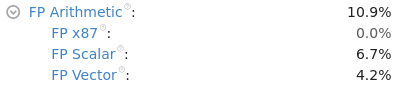
\includegraphics[width=0.5\textwidth, center]{reference_vtune.png}
        \caption{Reference}
    \end{figure}

    \begin{figure}[!htb]
        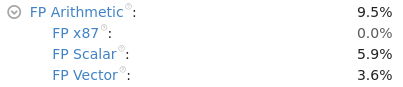
\includegraphics[width=0.5\textwidth, center]{associative-math_vtune.png}
        \caption{Associative-math}
    \end{figure}
\end{frame}

\subsection{Differences in the counters}

\begin{frame}[fragile]
    \frametitle{Differences in the counters}

    Difference with the reference (all counters):
    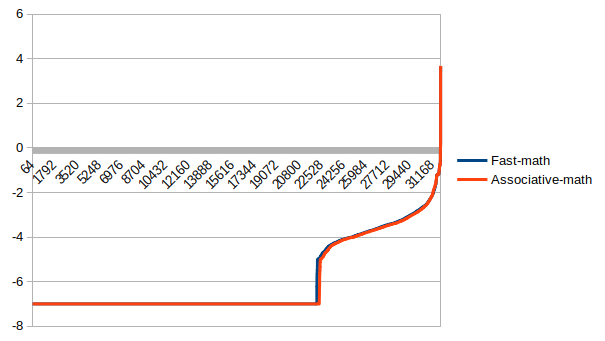
\includegraphics[width=\textwidth]{fast-math_difference.png}
\end{frame}

\part{Conclusion}

\section{Conclusion}

\begin{frame}[fragile]
    \frametitle{In a first time}

    \begin{itemize}
        \item Enabling \verb'-Wfloat-equal'.
        \item Enabling fast-math in one slot for instability checking.
              \begin{itemize}
                  \item Forget about \verb'finite-math-only' and \verb'unsafe-math-optimizations'.
              \end{itemize}
    \end{itemize}
\end{frame}

\begin{frame}[fragile]
    \frametitle{In a second time}

    \begin{itemize}
        \item Switch to fast-math for production.
              \begin{itemize}
                  \item Sometimes better precision (\emph{FMA} and \verb'double-precision-constant').
                  \item Coding clear equations and letting compiler optimize them.
                  \item GPU already using similar principles.
                  \item Dropping features that are legacies.
                  \item Assuming floats are approximations.
              \end{itemize}
    \end{itemize}
\end{frame}

\end{document}
